%%%%%%%%%%%%%%%%
% LaTeX Template
%%%%%%%%%%%%%%%%
\section{\texttt{LaTeX Template}}
\label{sec:latex_template}

The \texttt{LaTeX Template} folder is the topmost folder of this document. It contains the subfolders:
\begin{itemize}
    \item \hyperref[sec:images]{\texttt{Images}}
    \item \hyperref[sec:preamble]{\texttt{Preamble}}
    \item \hyperref[sec:sections]{\texttt{Sections}}
\end{itemize}
and contains the files:
\begin{itemize}
    \item \hyperref[sec:.gitignore]{\texttt{.gitignore}}
    \item \hyperref[sec:main.pdf]{\texttt{main.pdf}}
    \item \hyperref[sec:main.tex]{\texttt{main.tex}}
\end{itemize}

\subsection{\texttt{.gitignore}}
\label{sec:.gitignore}

The \texttt{.gitignore} file is not directly relevant to this \LaTeX\ template and can be safely ignored or removed. When compiling the \hyperref[sec:main.tex]{\texttt{main.tex}} file to produce the \hyperref[sec:main.pdf]{\texttt{main.pdf}} file, several auxiliary files are automatically generated to assist in the process. For the purpose of publishing this \LaTeX\ template to Github, it is not necessary to also publish these auxiliary files and it is preferable not to for the sake of a cleaner presentation. The \texttt{.gitignore} file is a list of files Git should ignore while tracking changes and publishing to Github.

You can read more about \texttt{.gitignore} \href{https://git-scm.com/docs/gitignore}{here}. For an introduction to Git, see \href{https://git-scm.com/book/en/v2}{here}. For an introduction to Github, see \href{https://skills.github.com/}{here}.

\subsection{\texttt{main.pdf}}
\label{sec:main.pdf}

You are currently reading the \texttt{main.pdf} file. This file is the end result of compiling the \hyperref[sec:main.tex]{\texttt{main.tex}} file.

\subsection{\texttt{main.tex}}
\label{sec:main.tex}

\lstinputlisting{main.tex}
For more information about the general structure of a \LaTeX\ document, see \href{https://en.wikibooks.org/wiki/LaTeX/Document_Structure#Global_structure}{here}.

%%%%%%%%
% Images
%%%%%%%%
\section{\texttt{Images}}
\label{sec:images}

The \texttt{Images} folder is exclusively intended to hold any image files you include in your document. Here is an example of how to include an image:
\begin{lstlisting}
\begin{center}
    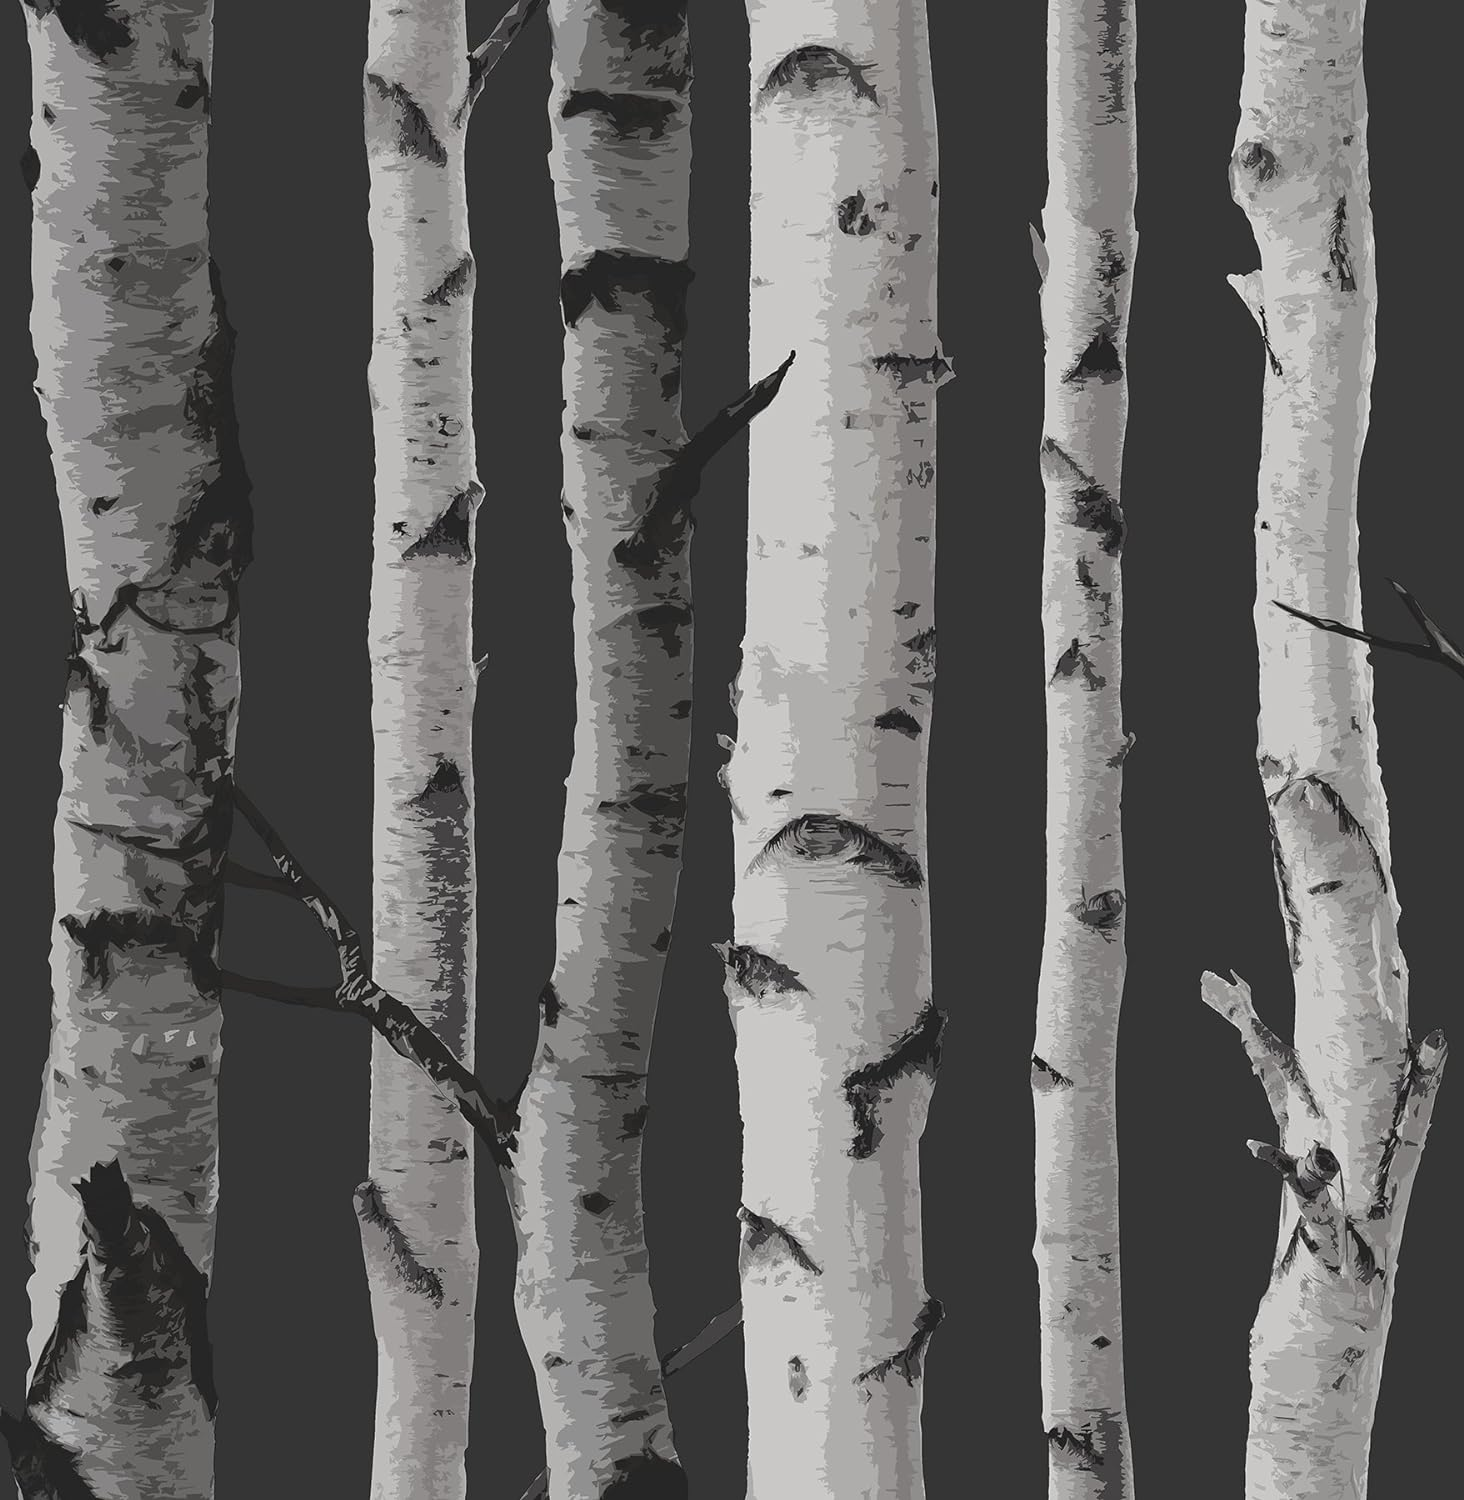
\includegraphics[width=0.5\linewidth]{birch.jpg}
\end{center}
\end{lstlisting}
This code renders the following:
\begin{center}
    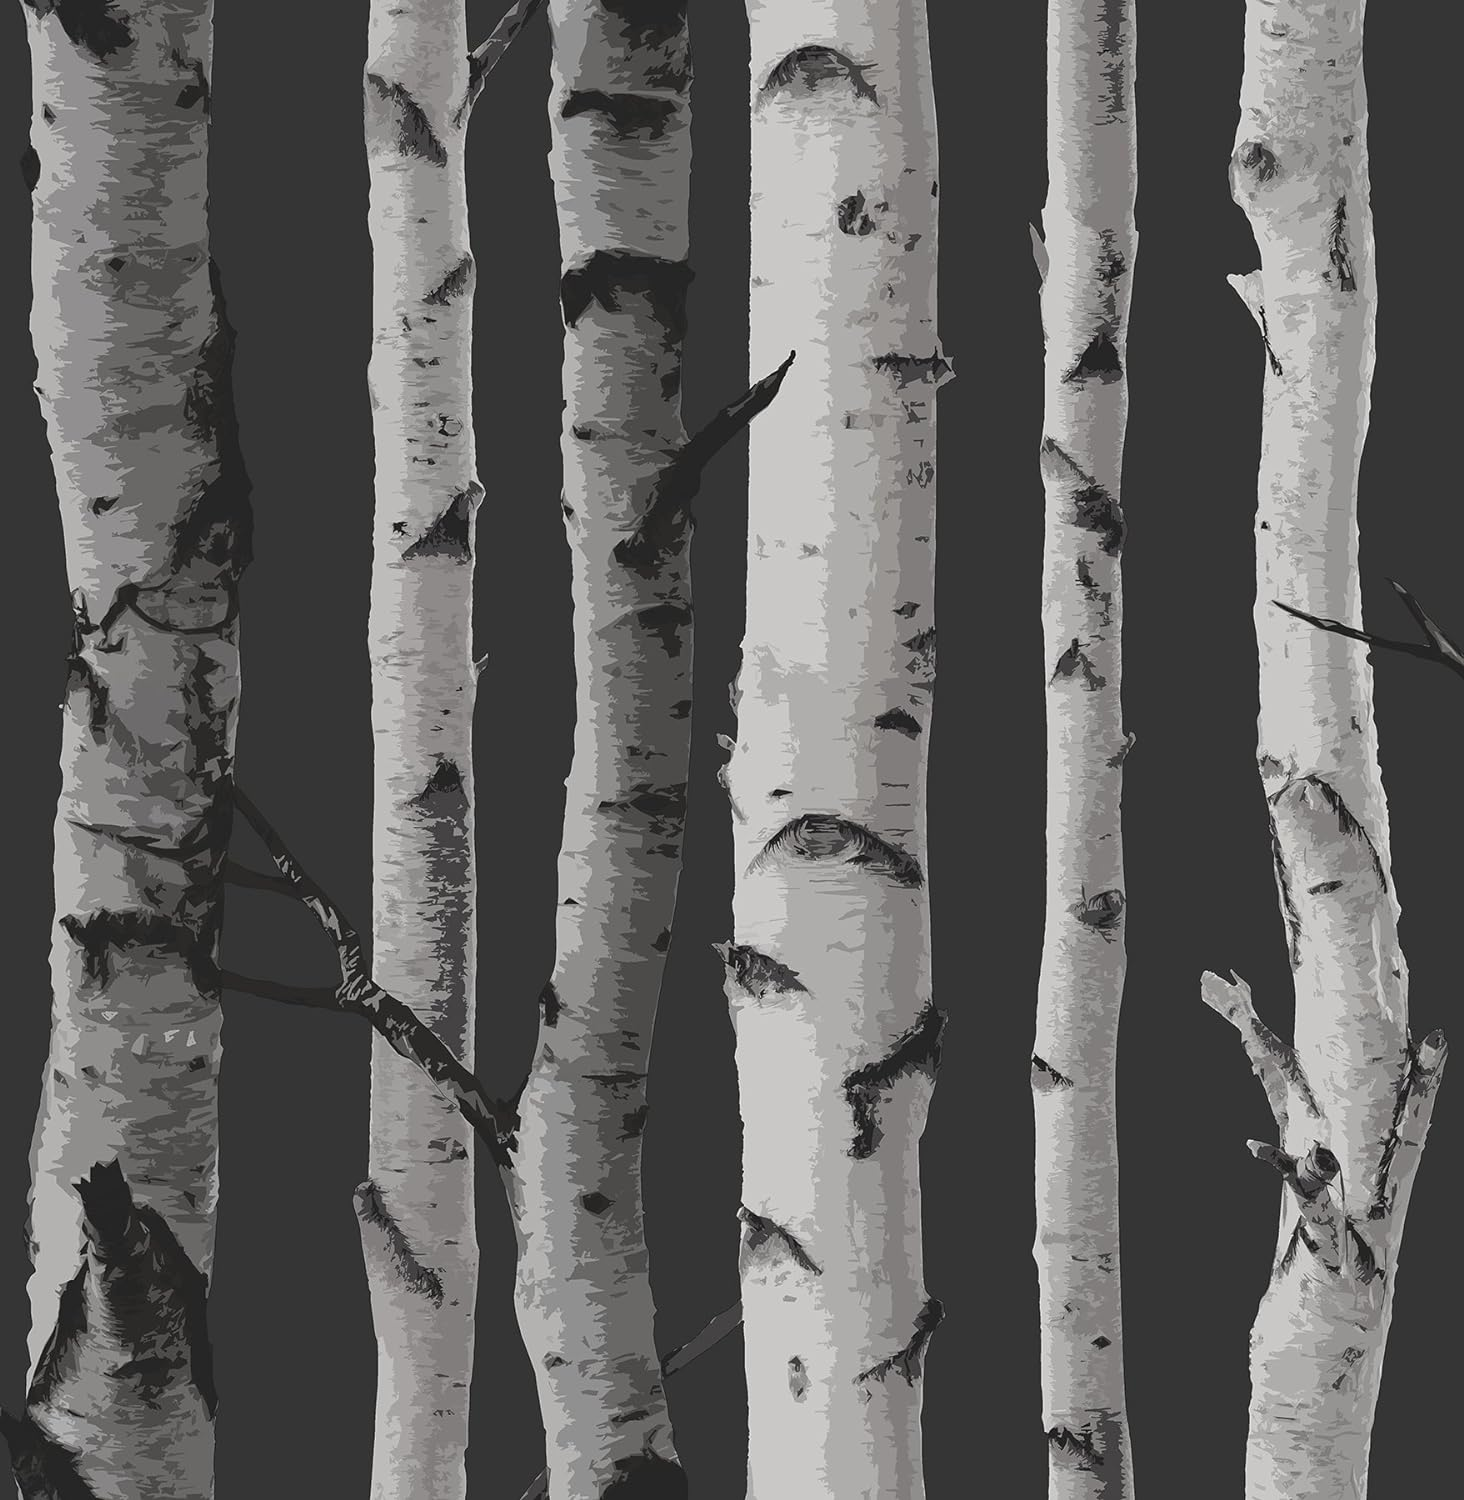
\includegraphics[width=0.5\linewidth]{birch.jpg}
\end{center}

The \lstinline|\includegraphics[<options>]{<file name>}| command is provided by the \texttt{graphicx} package which is internally loaded by the \texttt{tikz} package.

The \hyperref[sec:custom_settings.tex]{\texttt{custom\_settings.tex}} file includes the setting:
\begin{center}
    \lstinline|\graphicspath{{./Images/}}|
\end{center}
which establishes that \LaTeX\ should look for your image files in the \texttt{Images} folder by default.

For more information on including images in your document, see \href{https://en.wikibooks.org/wiki/LaTeX/Importing_Graphics}{here}.

%%%%%%%%%%
% Preamble
%%%%%%%%%%
\section{\texttt{Preamble}}
\label{sec:preamble}

The \texttt{Preamble} folder contains the files:
\begin{itemize}
    \item \hyperref[sec:packages.tex]{\texttt{packages.tex}}
    \item \hyperref[sec:custom_settings.tex]{\texttt{custom\_settings.tex}}
    \item \hyperref[sec:custom_commands.tex]{\texttt{custom\_commands.tex}}
    \item \hyperref[sec:environments.tex]{\texttt{environments.tex}}
    \item \hyperref[sec:header_footer.tex]{\texttt{header\_footer.tex}}
\end{itemize}
These files constitute the preamble of the document.

\subsection{\texttt{packages.tex}}
\label{sec:packages.tex}

\subsection{\texttt{custom\_settings.tex}}
\label{sec:custom_settings.tex}

\subsection{\texttt{custom\_commands.tex}}
\label{sec:custom_commands.tex}

\subsection{\texttt{environments.tex}}
\label{sec:environments.tex}

\subsection{\texttt{header\_footer.tex}}
\label{sec:header_footer.tex}

%%%%%%%%%%
% Sections
%%%%%%%%%%
\section{\texttt{Sections}}
\label{sec:sections}

\subsection{\texttt{static}}
\label{sec:static}

\subsubsection{\texttt{table\_of\_contents.tex}}
\label{sec:table_of_contents.tex}

\subsubsection{\texttt{appendix.tex}}
\label{sec:appendix.tex}

\subsubsection{\texttt{appendix\_lists.tex}}
\label{sec:appendix_lists.tex}

\subsection{\texttt{abstract.tex}}
\label{sec:abstract.tex}

\subsection{\texttt{body.tex}}
\label{sec:body.tex}

\subsection{\texttt{appendix\_body.tex}}
\label{appendix_body.tex}

